% ----------------------------------------
% Chapter: Stand der Technik
% ----------------------------------------
\chapter{Stand der Technik}
\label{chap:stand_der_technik}

Der Begriff Tribologie ist nach \cite{bartz_2000} die Wissenschaft und Technik von aufeinander einwirkenden Oberflächen in Relativbewegung.
Sie beschäftigt sich mit Reibung, Verschleiß und Schmierung sowie Grenzflächenwechselwirkungen zwischen Festkörpern, Flüssigkeiten und Gasen (Abbildung \ref{fig:das_tribologische_system}).

% ----------------------------------------
% Fig: Das tribologische System
% ----------------------------------------
\begin{figure}[htb]
    \centering
    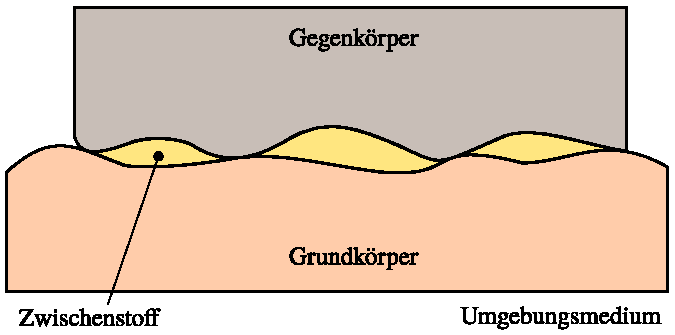
\includegraphics[]{./images/tribologisches_system.pdf}
    \caption{Das tribologische System\cite{wisniewski_2000}}
    \label{fig:das_tribologische_system}
\end{figure}

Die vorliegende Arbeit beschäftigt sich vornehmlich mit dem ölgeschmierten Kugel-Scheibe-Kontakt.
Aus diesem Grund soll im folgenden kurz auf die Themen Schmieröle, Reibung und auf die elastohydrodynamischen Grundlagen eingegangen werden.

% ----------------------------------------
% Sec: Eigenschaften des Schmiermittels
% ----------------------------------------
\section{Eigenschaften des Schmiermittels}
\label{sec:eigenschaften_des_schmiermittels}

% ----------------------------------------
% Subsec: Viskosität
% ----------------------------------------
\subsection*{Viskosität}
\label{sub:viskositaet}

Viskosität, die auch als innere Reibung bezeichnet wird, ist die wichtigste Kenngröße eines Schmierstoffes.
Sie beschreibt die Zähigkeit von Flüssigkeiten und Gasen.
Je größer die Viskosität ist, desto dickflüssiger ist das Fluid und umgekehrt.
Ein Modell des Parallelplattenversuchs veranschaulicht das Fließverhalten des Schmierstoffes (Abbildung \ref{fig:geschwindigkeitsprofil_parallelplattenversuch}).

% ----------------------------------------
% Fig: Geschwindigkeitsprofil in einem Parallelplattenversuch
% ----------------------------------------
\begin{figure}[htb]
    \centering
    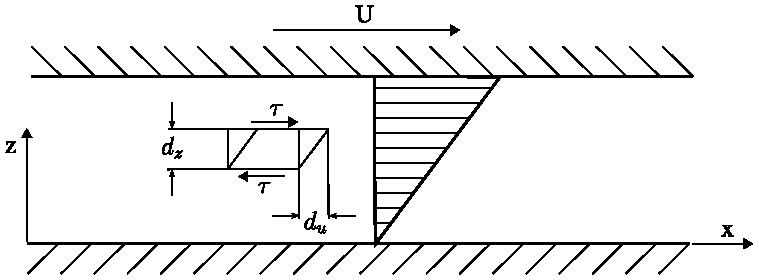
\includegraphics[]{./images/parallelplattenversuch.pdf}
    \caption{Geschwindigkeitsprofil in einem Parallelplattenversuch\cite{wisniewski_2000}}
    \label{fig:geschwindigkeitsprofil_parallelplattenversuch}
\end{figure}

Für die Newtonsche Flüssigkeit wird die Viskosität $\eta$ in Beziehung zu der Schubspannung $\tau$ definiert \cite{viscosity_wiki}:
% ----------------------------------------
% Eq: Viskosität
% ----------------------------------------
\begin{equation}
    \tau = \eta \cfrac{\partial u}{\partial z} \quad \text{oder} \quad \tau = \eta \dot{\gamma}
    \label{eq:viskositaet}
\end{equation}
%
wobei $u$ die Wälzgeschwindigkeit und $\gamma = u/z$ das Schergefälle ist.

Die kinematische Viskosität $\nu$ ergibt sich aus der dynamischen Viskosität $\eta$ durch die Division mit der Dichte des Fluids $\rho$.
Diese wird zur Charakterisierung des Fließverhaltens der Schmieröle verwendet.
% ----------------------------------------
% Eq: Kinematische Viskosität
% ----------------------------------------
\begin{equation}
    \nu = \frac{\eta}{\rho}
    \label{eq:kinematische_viskotitaet}
\end{equation}

Im Si-Einheitensystem hat die dynamische Viskosität $\eta$ die Einheit \si{N.s/m^2} oder \si{\pascal.\s} und die kinematische Viskosität $\nu$ die Einheit \si{m^2/s}.
Ein Stoff hat die Viskosität \SI{1}{N.s/m^2}, wenn er sich zwischen zwei Platten, die die Größe von \SI{1}{m^2} und einen Abstand von einander \SI{1}{m} haben, befindet und man \SI{1}{N} braucht, um die zwei Platten gegeneinander mit einer Geschwindigkeit von \SI{1}{m/s} zu verschieben \cite{viscosity_wiki}.

\subsection*{Temperatureffekt}
\label{sub:temperatureffekt}

Die Temperatur hat große Auswirkungen auf die Viskosität aller fließfähigen Stoffe.
Mit steigender Temperatur sinkt die Viskosität der Flüssigkeiten ab.
Dieser Effekt kann experimentell mittels eines Viskosimeters und rechnerisch nach \textit{Crouch} und \textit{Cameron} \cite{crouch_1961} bestimmt werden.

Die einfachste Gleichung, die den Temperatureffekt auf die Viskosität, nach \textit{Reynolds} \cite{reynolds_1886} beschreibt:
% ----------------------------------------
% Eq: Dynamische Viskosität nach Reynold
% ----------------------------------------
\begin{equation}
    \eta = \eta_{s}  \ exp \left( -\beta  \Delta\phi \right)
    \label{eq:dynamische_viskositaet_reynold}
\end{equation}
%
wobei $\eta_{s}$ die Viskosität des Schmierstoffes bei der Temperatur $\phi_{s}$ ist, $\eta$ ist die Viskosität des Schmierstoffes bei der Temperatur $\phi$, $\Delta{\phi}$ ist die Temperaturdifferenz ($\phi = \phi_{s} + \Delta{\phi}$) und $\beta$ ist die thermoviskose Konstante.

% ----------------------------------------
% Subsec: Viskositätsindex
% ----------------------------------------
\subsection*{Viskositätsindex}
\label{sub:Viskositaetsindex}

Die Temperaturabhängigkeit der kinematischen Viskosität eines Schmieröls wird mit dem Viskositätsindex (VI oder KVI) beschrieben.
Der Viskositätsindex basiert auf einer Skala, in der zwei unterschiedliche Öltypen mit deutlich abweichenden Viskositätstemperaturverhalten zugeordnet werden.
Das Öl, das starke Veränderungen der Viskosität zeigt, wird mit \num{0} oder \si{LVI} (low viscosity index) indiziert.
Das andere Öl wird mit \num{100} oder \si{HVI} (high viscosity index) gekennzeichnet.
Aus dem Vergleich der kinematischen Viskosität eines zu beschreibenden Öls mit diesen beiden Referenzölen bei \SI{100}{\degreeCelsius}  ergibt sich dessen Viskositätsindex nach Formel \ref{eq:viskositaetsindex}.
% ----------------------------------------
% Eq: Viskositätsindex
% ----------------------------------------
\begin{equation}
    VI~(oder KVI) = \frac{\nu_0 - \nu}{\nu_0 - \nu_{100}}
    \label{eq:viskositaetsindex}
\end{equation}

In der VI-Definition ist angenommen, dass die Veränderung der Viskosität mit der Temperatur von drei Ölen linear ist.
Die Linearisierung der kinematischen Viskosität $\nu$ von der Temperatur $\theta$ nach \textit{Walther (S\'{a}nchez-Rubio, et al.)} \cite{sanchez-rubio} lautet:
% ----------------------------------------
% Eq: kinematische Viskosität nach Walther
% ----------------------------------------
\begin{equation}
    \label{eq:kinematische_viskotitaet_walther}
    \log \log(\nu + 0,7) = A + B \log(\theta)
\end{equation}

Durch die Verwendung der doppeltlogarithmischen Koordinaten ergibt die Linearisierung für Mineralöle eine Gerade.
Abbildung \ref{fig:variation_der_viskositaet_mit_temperatur} zeigt ein Beispiel für die SAE-Öle.
Die Tabelle \ref{tab:esdu_oil_daten} und \ref{fig:fva_kin_viskositaet_temperatur} zeigen die Viskosität von verschiedenen Ölen bei unterschiedlichen Temperaturen.

% ----------------------------------------
% Fig: Variation der Viskosität mit der Temperatur
% ----------------------------------------
\begin{figure}[htb]
    \centering
    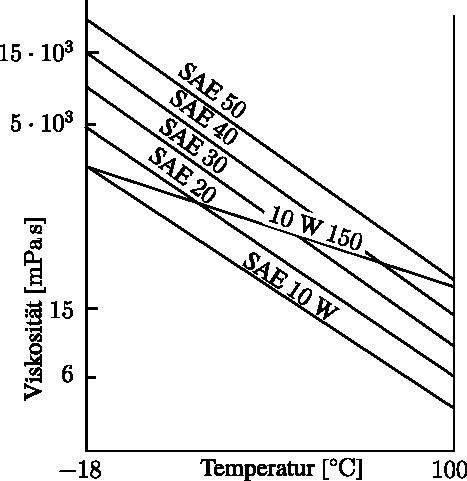
\includegraphics[]{./images/visko_temperatur.pdf}
    \caption{Variation der Viskosität mit Temperatur \cite{gohar_1988}}
    \label{fig:variation_der_viskositaet_mit_temperatur}
\end{figure}

% ----------------------------------------
% Subsec: Einfluss von Druck auf Viskosität
% ----------------------------------------
\subsection*{Einfluss von Druck auf Viskosität}
\label{sub:einfluss_von_druck_auf_viskositaet}

Mit steigendem Druck nimmt die Viskosität aller Schmieröle zu.
Allerdings verändert sich das Schmiermittel unter dem für die EHD-Kontakte enormen Druck schlagartig.
Die Viskosität nimmt rapide zu und der Schmierstoff erreicht einem festen Zustand.
Die Abbildung \ref{fig:dynamische_viskositaet_in_abhaengigkeit_vom_druck} zeigt, dass die Viskosität der FVA-Öle im Bereich von \SIrange{0}{200}{\mega\pascal} etwa hundertfach zunimmt.

% ----------------------------------------
% Fig: Viskosität - Druck - Verhalte
% ----------------------------------------
\begin{figure}[htb]
    \centering
    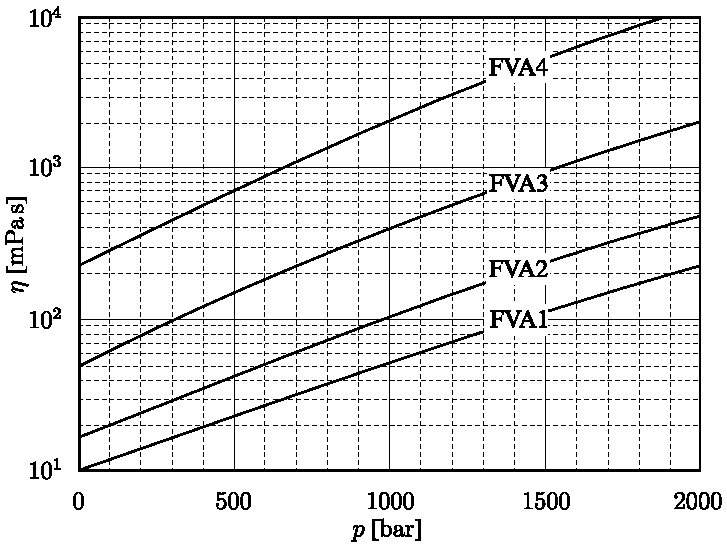
\includegraphics[]{./images/viskositaet_druck.pdf}
    \caption{Dynamische Viskosität der FVA-Referenzöle bei \SI{50}{\degreeCelsius} in Abhängigkeit vom Druck \cite{schilling_1985}}
    \label{fig:dynamische_viskositaet_in_abhaengigkeit_vom_druck}
\end{figure}
%

Nach \textit{Barus} \cite{cameron_1966} kann die Viskosität mit der unteren Formel berechnet werden,
% ----------------------------------------
% Eq: Viskositätsindex
% ----------------------------------------
\begin{equation}
    \eta = \eta_0 \ exp(\alpha p)
    \label{eq:dynamische_viskositaet_druck_barus}
\end{equation}
%
wobei $\eta_0$ die Viskosität beim Atmosphärendruck ($p =  0$) und $\alpha_p$ der Druck-Viskosität-Koeffizient  ist.
Für Mineralöle sind diese Parameter ungefähr \cite{wisniewski_2000}:

\begin{tabular}{lll}
    \num{0,001} $\rightarrow$ \num{0,1} & für & $\eta_0$ [\si{\pascal.\second}] \\
    \num{0} $\rightarrow$ \num{2.0e-8}  & für & $\alpha$ [\si{\per\pascal}]
\end{tabular}

Leider liefert die Gleichung von \textit{Barus} einen zu großen Wert bei hohem Druck.
Eine genauere Gleichung für die Viskosität bei der Temperatur $\theta$ wurde von \textit{Roelands} \cite{roelands} vorgeschlagen:
% ----------------------------------------
% Eq: Roelands Gleichung
% ----------------------------------------
\begin{equation}
    \eta_R = \eta_0 \ exp (\alpha^* p)
    \label{eq:dynamische_viskositaet_druck_roelands}
\end{equation}
%

Der \textit{Roelands} Druck-Viskositätskoeffizient $\alpha^*$ ist eine Funktion des Drucks $p$ und der Temperatur $\theta$ und kann mit Formel \ref{eq:roelands_alpha} berechnet werden:
% ----------------------------------------
% Eq: Roelands Druck-Viskositätskoeffizient
% ----------------------------------------
\begin{equation}
    \alpha^* p = [\ln(\eta_0) + 9.67]
                 \left\{
                 \left( \cfrac{\theta - 138}{\theta_0 - 138} \right ) ^{-S_0}
                 \left[
                     \left ( 1 + \cfrac{p}{p_0} \right ) ^ Z
                     - 1 
                 \right]
                 \right\}
    \label{eq:roelands_alpha}
\end{equation}
%
wobei $\theta_0$ [\si{\kelvin}] die Raumtemperatur umd $p_0 =$ \SI{1.98e8}{\pascal} eine Konstante ist.
Die $Z$ und $S_0$ sind die Konstanten für alle Öle, unabhängig von Temperatur und Druck und können durch die unteren Formeln \cite{gohar_1988} berechnet werden:
% ----------------------------------------
% Eq: Roelands Gleichung Parameters
% ----------------------------------------
\begin{align}
    Z &= \cfrac{\alpha}{5.1 \times 10^9 (\log(\eta_0) + 9.67)} \\
    S_0 &= \cfrac{\beta (\theta_0 - 138)}{\log(\eta_0) + 9.67}
\end{align}
%
$\alpha$ und $\beta$ sind für bekannte Öle gegeben (siehe Tabelle \ref{tab:esdu_oil_daten} für $\alpha$).
Zum Berechnungszwecken wird $Z =$ \num{0.68} genommen.

Der Viskositäts-Druck-Koeffizient $\alpha$ ist keine Konstante, sondern eine Funktion der Temperatur.
Die Abbildung \ref{fig:druckkoeffizient_temperatur} zeigt diese Abhängigkeit im Bereich von \SIrange{0}{2000}{\bar} (Index \num{2000}) mit der Temperatur für die Referenzöle der FVA an.

% ----------------------------------------
% Fig: Druckkoeffizient der FVA-Referenzöle in Abhängigkeit von der Temperatur
% ----------------------------------------
\begin{figure}[htb]
    \centering
    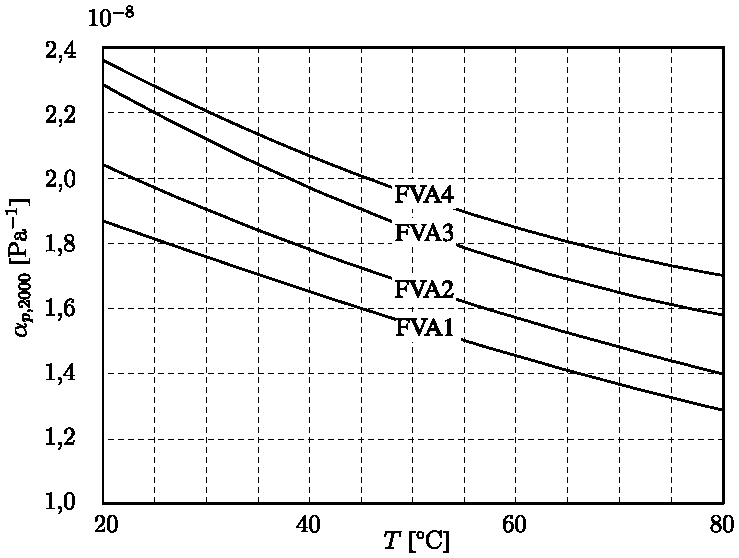
\includegraphics[]{./images/visko_druck_koeffizient.pdf}
    \caption{Viskositäts-Druck-Koeffizient der FVA-Referenzöle in Abhängigkeit von der Temperatur \cite{schilling_1985}}
    \label{fig:druckkoeffizient_temperatur}
\end{figure}

% ----------------------------------------
% Subsec: Dichte
% ----------------------------------------
\subsection*{Dichte}
\label{sub:dichte}

Für eine numerische Schmierfilmdickenmessung ist es notwendig zu wissen, wie sich die Dichte des Schmierstoffes unter variierendem Drucken verhält.
Die Form des Schmierfilms kann nicht richtig berechnet werden, wenn diese Eigenschaft vernachlässigt wird.
Die Kompressibilität eines Schmierstoffes $C$ kann nach \textit{Chu} und \textit{Cameron} \cite{chu_1962} so beschrieben werden:
% ----------------------------------------
% Eq: Die Kompressibilität eines Schmierstoffes
% ----------------------------------------
\begin{equation}
    \label{eq:kompressibilitaet}
    C = \left( \frac{1}{\rho} \right) \frac{d\rho}{dp} = \left( \frac{1}{V} \right) \frac{dV}{dp}
\end{equation}
%
wobei $V$ das Volumen und $dV$ die Änderung des Volumens ist.

Die Dichte der Mineralöle ist nach \textit{Dowson} und \textit{Higginson} \cite{dowson_1966} mit folgender Formel zu berechnen:
% ----------------------------------------
% Eq: Dichte nach Dowson und Higginson
% ----------------------------------------
\begin{equation}
    \label{eq:dichte_dowson_higginson}
    \rho = \rho_0 \left( 1 + \frac{0,6  p}{1 + 1,7  p} \right)
\end{equation}
%
wobei $p$ der Druck und $\rho_0$ die Dichte bei normalem Luftdruck (\SI{0,87}{kg/m^3} bei \SI{20}{\degreeCelsius}) ist.
Abbildung \ref{fig:variation_der_dichte_bei_verschiedenen_druecke} zeigt einen Plot der Gleichung \ref{eq:dichte_dowson_higginson} für ein Mineralöl, das eine Dichte $\rho_0$ von \num{0.85} bei \SI{40}{\degreeCelsius} hat.
Die Messpunkte $\triangle$ stammen aus Versuchen von \textit{Hirano et al} \cite{hirano}.

% ----------------------------------------
% Fig: Druckkoeffizient der FVA-Referenzöle in Abhängigkeit von der Temperatur
% ----------------------------------------
\begin{figure}[htb]
    \centering
    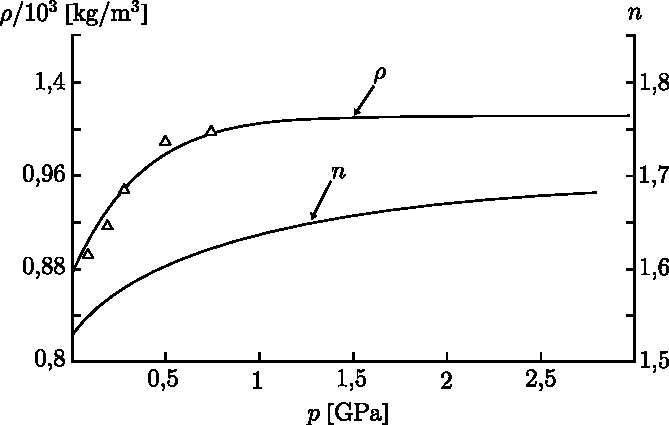
\includegraphics[]{./images/dichte_brechungsindex_temperatur.pdf}
    \caption{Variation der Dichte und des Brechungsindexs bei unterschiedlichem Drücken \cite{gohar_1988}}
    \label{fig:variation_der_dichte_bei_verschiedenen_druecke}
\end{figure}

% ----------------------------------------
% Subsec: Brechungsindex
% ----------------------------------------
\subsection*{Brechungsindex}
\label{sub:brechungsindex}

Für die Messverfahren, die auf optischen Interferometrie basieren, braucht man die Abhängigkeit zwischen der Dichte und dem Brechungsindex des Schmierstoffes.
Nach \textit{Gohar} \cite{gohar_1966} wird das Verhältnis mit der Formel~\ref{eq:dichte_brechnungsindex} beschrieben:
% ----------------------------------------
% Eq: Dichte und Brechungsindex
% ----------------------------------------
\begin{equation}
    \label{eq:dichte_brechnungsindex}
    c\rho = \frac{n^2 - 1}{n^2 + 2}
\end{equation}
%
wobei $c$ ein Ölkonstante (zB: SAE-30, $c = $ \num{0.33}) ist.
Der Brechungsindex beträgt für die meisten Mineralöle bei normalen Luftdruck ca. \num{1.51}.
Die Abhängigkeit des Brechungsindexs von dem Druck für das Öl SAE-30 wird auch in die Abbildung \ref{fig:variation_der_dichte_bei_verschiedenen_druecke} angezeigt.

% ----------------------------------------
% Subsec: Wärmeleitfähigkeit
% ----------------------------------------
\subsection*{Wärmeleitfähigkeit}
\label{waermeleitfaehigkeit}

Um die Temperaturerhöhung des Schmierstoffes unter Schubspannung zu schätzen, ist dessen Wärmeleitfähigkeit $k$ nötig.
Nach \textit{Cameron} \cite{cameron_1966} kann diese Größe bei normalem Luftdruck mit folgender Formel berechnet werden.
% ----------------------------------------
% Eq: Wärmeleitfähigkeit
% ----------------------------------------
\begin{equation}
    \label{eq:waermeleitfaehigkeit}
    k = \frac{0,1173 - 6,33 \times 10^{-5} \ \theta}{\rho_0}
\end{equation}
%
wobei $\theta$ [\si{\kelvin}] die absolute Temperatur und $\rho_0$ [\si{kg/m^3}] die Dichte ist.

% ----------------------------------------
% Subsec: Newtonsche Fluide
% ----------------------------------------
\subsection*{Newtonsche Fluide}
\label{sub:newtonsche_fluide}

Wenn die Viskosität eines Fluids von der Schubspannung unabhängig ist, wird das Fluid als Newtonsches Fluid bezeichnet (siehe Abbildung\ref{fig:newtonsche_fluide}).
Flüssigkeiten, deren Viskosität mit steigenden Schubspannungen zunimmt, nennt man dilatant.
Solches Verhalten zeigt häufig Suspensionen an, die nicht als Schmierstoff sich eigen.
Strukturviskose Fluide sind die Umkehr der Dilatanz.
Strukturviskosität tritt bei synthetischen Fluiden auf.
Für die Bestimmung der Schmierfilmdicke werden alle Fluide in Rahmen dieser Arbeit als Newtonsche Fluide angenommen.

% ----------------------------------------
% Fig: Newtonsche und nicht newtonsche Fluide
% ----------------------------------------
\begin{figure}[htb]
    \centering
    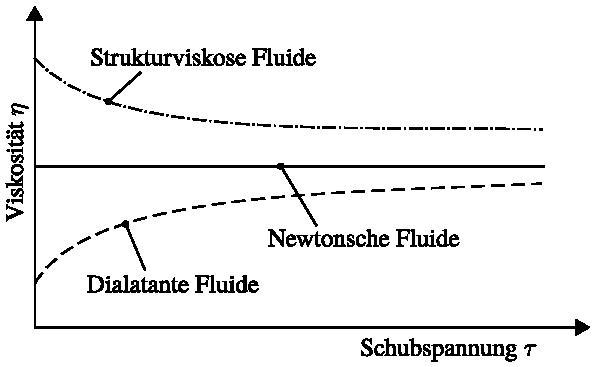
\includegraphics[]{./images/newtonsche_nichtnewtonsche_fluide.pdf}
    \caption{Newtonsche und die andere Fluide\cite{wisniewski_2000}}
    \label{fig:newtonsche_fluide}
\end{figure}
%

% ----------------------------------------
% Sec: Reibung
% ----------------------------------------
\section{Reibung}
\label{sec:reibung}

% ----------------------------------------
% Subsec: Reibungsarten
% ----------------------------------------
\subsection{Reibungsarten}
\label{sub:reibungsarten}

Bewegungsreibung ist immer da, wo sich berührende Körper bzw. Stoffbereiche relativ zueinander bewegen.
Sie ist entgegen der Bewegungsrichtung gerichtet und wandelt die mechanische Energie in Wärme.
Man unterscheidet zwischen innerer und äußerer Reibung.
Äußere Reibung tritt auf, wo die Flächen der unterschiedlichen Körpern sich berühren.
Von innerer Reibung spricht man, wenn die sich berührenden Stoffbereiche einem Körper angehören, z.B im Schmierstoff.

Im Gegensatz zur Bewebungsreibung tritt die Haftreibung auf, wo es keine relative Bewegung zwischen den Reibpartnern gibt.
In diesem Fall ist die angreifende Kraft nicht ausreichend, um die Körper in Bewegung zu bringen.

Reibung wird durch den Reibwert $\mu$ charakterisiert.
Er beschreibt das Verhältnis von der Reibungskraft $F_R$ und der Normalkraft $F_N$ \cite{reibung}:
% ----------------------------------------
% Eq: Reibung
% ----------------------------------------
\begin{equation}
    \label{eq:reibung}
	\mu = \cfrac{F_R}{F_N}
\end{equation}
%

Die Bewegungsreibung kann man zu drei Kategorien --- Gleitreibung, Rollreibung und Bohrreibung --- einteilen (siehe Abbildung \ref{fig:arten_der_bewegungsreibung}).
In der Praxis treten meist Kombinationen dieser drei Reibungsarten auf.
Die wichtigste ist hier die sogenante Wälzreibung, eine Kombination aus Rollen und Gleiten.
% ----------------------------------------
% Fig: Arten der Bewegungsreibung
% ----------------------------------------
\begin{figure}[htb]
    \centering
    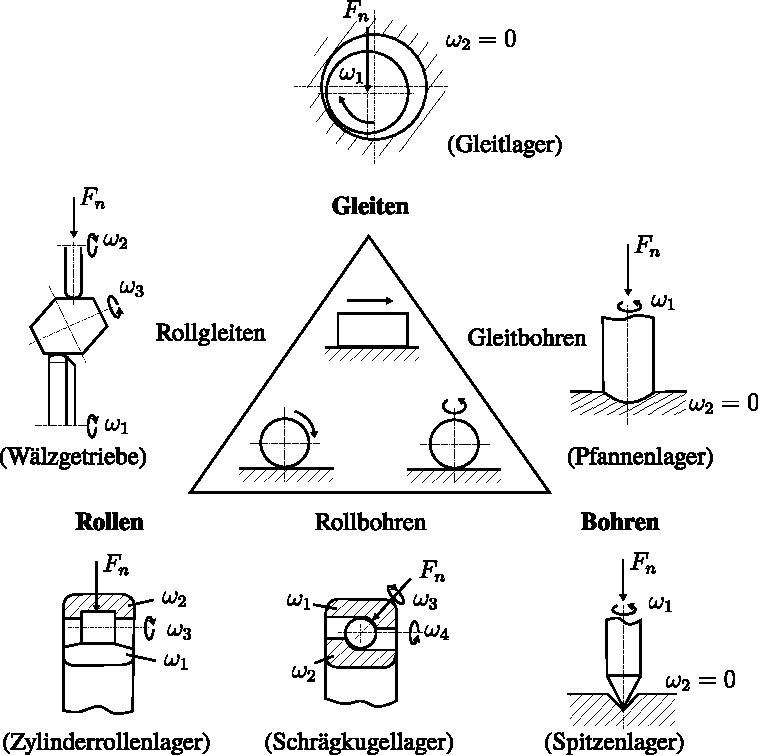
\includegraphics[]{./images/bewegungsarten.pdf}
    \caption{Arten der Bewegungsreibung \cite{steinhilper_2008}}
    \label{fig:arten_der_bewegungsreibung}
\end{figure}
%

% ----------------------------------------
% Subsec: Reibungszustände und Schmierfilmaufbau
% ----------------------------------------
\subsection{Reibungszustände und Schmierfilmaufbau}
\label{sub:reibungszustaende_und_schmierfilmaufbau}

Die Reibungszustände werden durch den Kontaktzustand der beteiligten Reibpartner beschrieben.
Man spricht hier von Festkörper-, Grenz-, Misch-, Flüssigkeits- und Gasreibung.
Da die Gasreibung für diese Arbeit unrelevant ist, wird kurz auf die einzelnen Reibungszustände ohne Gasreibung eingegangen.

% ----------------------------------------
% Par: Festkörperreibung
% ----------------------------------------
\paragraph{Festkörperreibung:}
\label{par:festkoerperreibung}
%
\begin{wrapfigure}{R}{0.25\textwidth}
    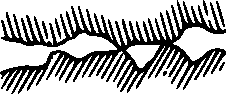
\includegraphics[trim={0 1cm 0 1cm}]{./images/festkoerperreibung.pdf}
\end{wrapfigure}

Von Festkörperreibung spricht man, wenn sich kein Schmierstoff im Reibkontakt befindet.
Dabei besteht bei hohen Flächenpressungen die Gefahr , dass die beiden Körper aneinander haften, verschleißen und es zum Festfressen kommen kann.

% ----------------------------------------
% Par: Grenzreibung
% ----------------------------------------
\paragraph{Grenzreibung:}
\label{par:grenzreibung}
%
\begin{wrapfigure}{R}{0.25\textwidth}
    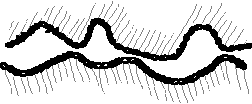
\includegraphics[trim={0 0.5cm 0 0.5cm}]{./images/grenzreibung.pdf}
\end{wrapfigure}

Grenzreibung ist der Festkörperreibung recht ähnlich.
Allerdings werden die Oberflächen der Reibpartner von einer Schicht getrennt und befinden sich nicht direkt in Berührung.
Diese Schicht kann zum Beispiel durch Oxidation, Adsorption oder chemische Reaktionen entstanden sein und vermindert die Reibung im Verleich zur Festkörperreibung schon eheblich.

% ----------------------------------------
% Par: Mischreibung
% ----------------------------------------
\paragraph{Mischreibung:}
\label{par:mischreibung}
%
\begin{wrapfigure}{R}{0.25\textwidth}
    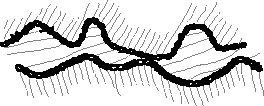
\includegraphics[trim={0 0.5cm 0 0.5cm}]{./images/mischreibung.pdf}
\end{wrapfigure}

Bei Mischreibung gibt es schon im Reibkontakt ein bisschen Schmierstoff und die Laufflächen werden zum Teil durch einen Schmierfilm getrennt.
Leider ist dieser nicht hoch genug, um ein vollständiges Trennen der beiden Körpern zu erreichen.
Es kommt immer noch zu einer Berührung der Rauheitsspitzen der Laufflächen.
Die Reibung bei der Mischreibung ist deutlich geringer als die der Grenzreibung. Allerdings bleibt immer noch der Verschleiß im Reibkontakt.

% ----------------------------------------
% Par: Flüssigkeitsreibung
% ----------------------------------------
\paragraph{Flüssigkeitsreibung:}
\label{par:fluessigkeitsreibung}
%
\begin{wrapfigure}{R}{0.25\textwidth}
    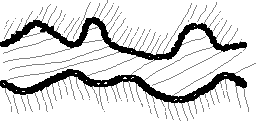
\includegraphics[trim={0 0.5cm 0 0.5cm}]{./images/fluessigkeitreibung.pdf}
\end{wrapfigure}

Bei Flüssigkeitsreibung handelt sich um eine vollständige Trennung der Laufflächen.
Selbst die Rauheitsspitzen berühren sich hierbei nicht mehr.
Die äußere Reibung ist weg, so dass nur noch die innere Reibung bleibt, die durch die Scherbeanspruchung des Schmierstoffs hervorgerufen wird.

Der Aufbau des Schmierfilms erfolgt hydrodynamisch, elastohydrodynamisch oder hydrostatisch.
Hydrostatisch aufgebaute Schmierfilme werden durch externe Aggregate, wie zum Beispiel eine Pumpe, aufgebaut.
Bei der hydrodynamischen Schmierung wird der Schmierfilm durch die Relativbewegung der Reibpartner aufgebaut.
Die hydrodynamische Schmierung tritt im Allgemein nur bei konformen Kontaktpaarungen auf.
Bei konformen Kontaktpaarungen spricht man von Kontaktkörpern, die sich auf einer Fläche berühren.
Eine Verformung der Oberflächen spielt hier keine wichtige Rolle, da die Pressungen aufgrund der großen Kontaktflächen vergleichsweise gering sind.
Im Gegenteil dazu ist bei der elastohydrodynamischen Schmierung die Flächenpressung ein entscheidender Faktor zum Aufbau einer tragenden Schicht.
Die Kontaktpaarungen bei dieser Schmierung sind im Allgemein kontraform.
Ihre Flächen berühren sich nur in einem Punkt oder in einer Linie.
Dadurch treten deutlich höhere Flächenpressungen als bei konformen Kontakten auf, was zu einer lokalen Verformung der Oberflächen führt.
Durch dieses Phänomen und die Zunahme der Viskosität des Schmierstoffes unter hohem Druck wird der Schmierfilm im Kontaktbereich bei elastohydrodynamischen Schmierung aufgebaut.

% ----------------------------------------
% Par: Stribeck-Kurve
% ----------------------------------------
\subsection{Stribeck-Kurve}
\label{sub:stribeck-kurve}

Zur anschaulichen Darstellung der verschiedenen Reibungszustände wird häufig die Stribeck-Kurve gewählt.
In die Abbildung \ref{fig:stribeck-kurve} wird die Reibungszahl eines geschmierten Gleitlagers in Abhängigkeit von der Geschwindigkeit dargestellt.

% ----------------------------------------
% Fig: Stribeck-Kurve
% ----------------------------------------
\begin{figure}[htb]
    \centering
    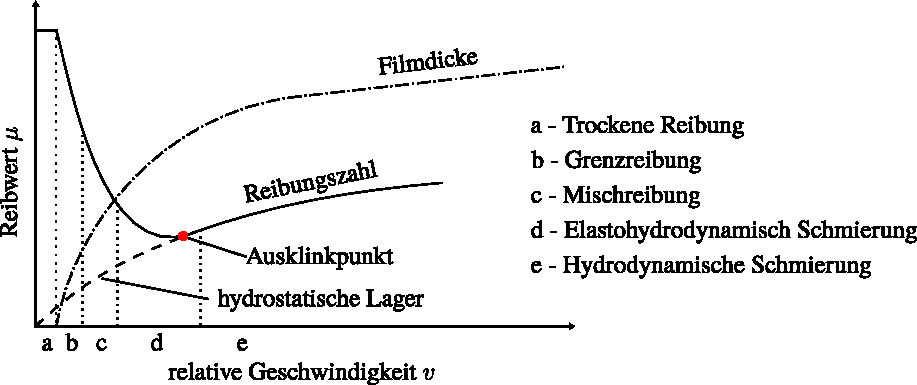
\includegraphics[]{./images/stribeckkurve.pdf}
    \caption{Stribeck-Kurve eines geschmierten Gleitlagers \cite{ikz_haustechnik}}
    \label{fig:stribeck-kurve}
\end{figure}
%

Im Stillstand tritt erst einmal reine Haftreibung auf.
Nach dem Anlauf des Lagers sinkt die Reibungszahl trotz des fehlenden Schmierstoffes im Reibkontakt und es kommt zur Grenzreibung.
Mit zunehmender Relativgeschwindigkeit zwischen Lagerbuchse und Welle wird der Schmierstoff in den Lagerspalt befördert.
Jetzt nimmt die Reibung weiter ab und es kommt zur Mischreibung.
Bei weiter zunehmender Drehzahl sinkt die Reibungszahl ab bzw. steigt der Schmierfilm weiter an bis es ab dem Ausklinkpunkt zur reinen Flüssigkeitsreibung kommt.
Nun schwimmt die Welle im Schmierstoff und berührt nicht mehr die Lagerbuchse.
Da die innere Reibung mit der steigenden Drehzahl zunimmt, liegt an der Stelle (Ausklinkpunkt) ein Minimum der Reibungszahl vor.

Für Gleitlager, deren Schmierfilm hydrostatisch durch eine Pumpe aufgebaut wird, gilt die Stribeck-Kurve nicht.
Da der Schmierfilm schon beim Stillstand voll ausgebildet ist, befinden sich solche Lager bei jeder Drehzahl im Bereich der Flüssigkeitsreibung.

% ----------------------------------------
% Sec: Betrachtung des EHD-Kontaktes
% ----------------------------------------
\section{Betrachtung des EHD-Kontaktes}
\label{sec:betrachtung_des_ehd_kontaktes}

Die Kontaktflächen von Maschinenelementen werden in zwei Grundformen eingeteilt.
Dieses sind konforme (zB. Gleitlager) und nichtkonforme Paarungen (z.B. Zahnrad, Reibrad, Nocken-Stößel).
Die Abbildung~\ref{fig:konforme_kontraforme_kontakte} zeigt die Beispiele konformer und nichtkonformer Kontakte an.

% ----------------------------------------
% Fig: Nichtkonforme Paarungen
% ----------------------------------------
\begin{figure}[htb]
    \centering
    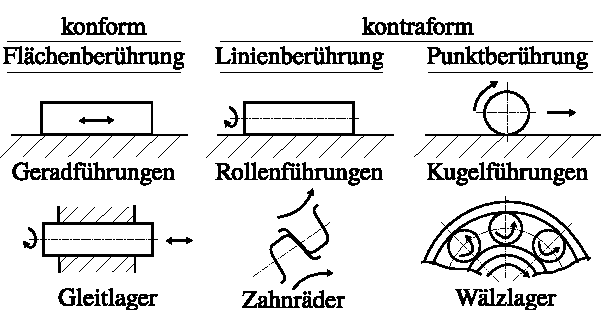
\includegraphics[]{./images/konforme_kontraforme_kontakte.pdf}
    \caption{Konforme und kontraforme Kontakte \cite{steinhilper_2008}}
    \label{fig:konforme_kontraforme_kontakte}
\end{figure}

Im Gegenteil zu den konformen Kontakten, wo die Pressungen in der Größenordnung von \SI{10}{\mega\pascal} auftreten, können --- in zwischen den Laufflächen nichtkonforme Kontakte --- die Druckspannungen von \SI{0.5}{\giga\pascal} und höher betragen.
Durch die enorme, konzentrierte Belastung werden die Flächen an dem Kontaktpunkt elastisch verformt und vergrößert.
Im Folgenden soll der Wälzkontakt nach \textit{Wisniewski} \cite{wisniewski_2000} näher betrachtet werden.

\subsection{Kontakt von beliebig gekrümmten Elementen}
\label{sub:kontakt_von_beliebig_gekruemmten_elementen}

Bei der Betrachtung des konzentrischen Kontaktes werden alle Oberflächen als ideal glatt angenommen.
Durch deren minimale und maximale Krümmungen wird die Geometrie des Grundkörpers bzw. des Gegenkörpers beschrieben.
Bei konvexen Körpern (Index 1) sind die Krümmungsradien ($r_{11}, r_{12}$) positiv und bei konkaven Körpern (Index 2) sind die Radien ($r_{21}, r_{22}$) negativ.
Zwischen den beiden Ebenen, die $r_{11}$ und $r_{21}$ erhalten, bildet sich der Winkel $\varphi$.
In Abbildung~\ref{fig:kontaktgeometrie_nichtkonforme_kontakte} wird die generelle Kontaktgeometrie bei nicht konformen Festkörpern dargestellt.

% ----------------------------------------
% Fig: Wälzkontakt nach Wisniewski
% ----------------------------------------
\begin{figure}[htb]
    \centering
    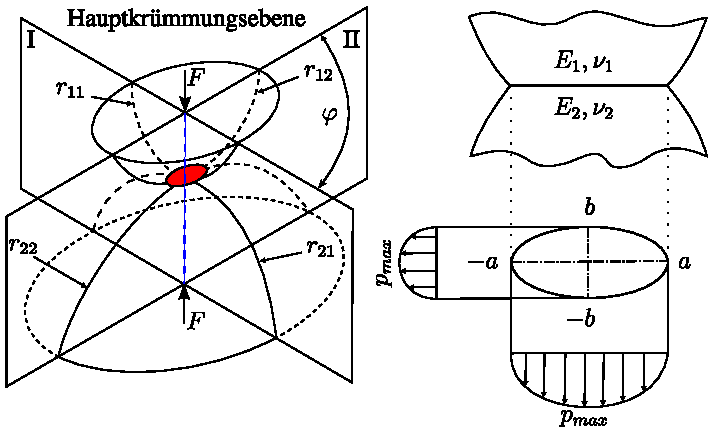
\includegraphics[width=0.8\textwidth]{./images/hertzsche_pressung.pdf}
    \caption{Kontaktgeometrie bei nicht konformer Paarungen\cite{psm}}
    \label{fig:kontaktgeometrie_nichtkonforme_kontakte}
\end{figure}

Im Kontaktpunkt bildet die Kontaktfläche eine Ellipse mit den Halbachsen $a$ und $b$.
Um $a$ und $b$ zu bestimmen, braucht man das reduzierte Elastizitätsmodul $E$, die Belastung $P$ und der Krümmungsradius $R$.
% ----------------------------------------
% Eq: Laengen der Halbachsen der Kontaktellipse
% ----------------------------------------
\begin{align}
    a = \beta_a  \sqrt[3]{\frac{3  P  R}{E}} \label{eq:laenge_a} \\
    b = \beta_b  \sqrt[3]{\frac{3  P  R}{E}} \label{eq:laenge_b}
\end{align}

Das reduzierte Elastizitätsmodul $E'$ beschreibt die elastische Eigenschaften der beiden Elemente und wird definiert als
% ----------------------------------------
% Eq: Der reduzierte Elastizitätsmodul E
% ----------------------------------------
\begin{equation}
    \label{eq:reduzierter_elastizitaetsmodul}
    \frac{1}{E'} = \frac{1}{2}  \left( \frac{1 - \nu_1^2}{E_1} + \frac{1 - \nu_2^2}{E_2} \right)
\end{equation}
%
wobei $\nu_x$ die Querkontraktionszahl der Kontaktkörper und $E_x$ der Elastizitätsmodul der Kontaktkörpern ist.
Die Druckverteilung $p$ hat die Form eines Halbellipsoids und wird so definiert:
% ----------------------------------------
% Eq: Druckverteilung p
% ----------------------------------------
\begin{equation}
    \label{eq:druckverteilung}
    p = p_0  \sqrt{1 - \left( \frac{x}{b} \right)^2 - \left( \frac{y}{a} \right)^2}
\end{equation}
%
wobei $x$ und $y$ die Koordinaten in der Ebene ist.
Die maximale Pressung $p_0$ ist ein Produkt der Belastung $P$ und der Länge von Halbachsen $a$ und $b$ sind.
% ----------------------------------------
% Eq: Maximale Pressung p0
% ----------------------------------------
\begin{equation}
    \label{eq:maximale_pressung}
    p_0 = \frac{3  P}{2  \pi  a  b}
\end{equation}
%
Der reziproke Krümmungsradius $R$ wird mit der Summe aller vier Hauptkrümmungen $r_x$ bestimmt
% ----------------------------------------
% Eq: Krümmungsradius R
% ----------------------------------------
\begin{equation}
    \label{eq:kruemmungsradius}
    \frac{1}{R} = \frac{1}{r_{11}} + \frac{1}{r_{12}} + \frac{1}{r_{21}} + \frac{1}{r_{22}}
\end{equation}
%
Die Koeffizienten $\beta_a$ und $\beta_b$ zur Bestimmung der Berührungsfläche in einem konformen Kontakt können über den Parameter $\cos{\psi}$ aus dem Diagram \ref{fig:beta_a_und_beta_b_als_funktion_der_cos_psi} abgelesen werden.

% ----------------------------------------
% Fig: beta_a und beta_b als Funktion des cos_psi
% ----------------------------------------
\begin{figure}[htb]
    \centering
    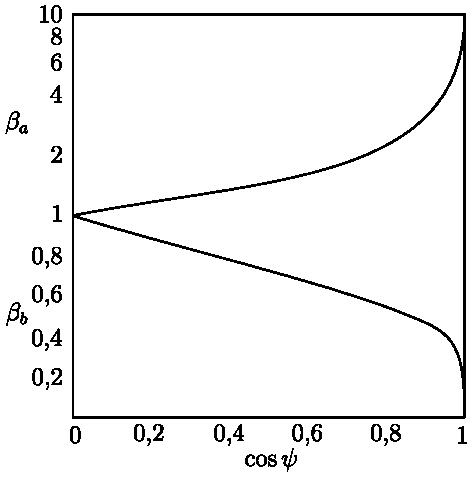
\includegraphics[]{./images/beta_cos_psi_diagram.pdf}
    \caption{$\beta_a$ und $\beta_b$ als Funktion von $\cos{\psi}$\cite{wisniewski_2000}}
    \label{fig:beta_a_und_beta_b_als_funktion_der_cos_psi}
\end{figure}
%

Der Parameter $\cos{\psi}$ kann mit folgender Formel \ref{eq:cos_psi} berechnet werden:
% ----------------------------------------
% Eq: cos psi
% ----------------------------------------
\begin{equation}
    \label{eq:cos_psi}
    \cos{\psi} = R  \sqrt{\left( \frac{1}{r_{11}} - \frac{1}{r_{12}} \right)^2 
                                + \left( \frac{1}{r_{21}} - \frac{1}{r_{22}} \right)^2 
                                + 2  \cos{2 \varphi} 
                                 \left( \frac{1}{r_{11}} - \frac{1}{r_{12}}  \right)^2 
                                 \left( \frac{1}{r_{21}} - \frac{1}{r_{22}} \right)^2}
\end{equation}


Für ein Kugel-Scheibe-Modell gilt

% ----------------------------------------
% Eq: Radius der Kugel und Scheibe im Kugel-Scheibe-Modell
% ----------------------------------------
\begin{align*}
    r_{11} &= r_{12} = r_{Kugel} \\
    r_{21} &= r_{22} = r_{Scheibe} = \infty
\end{align*}


% ----------------------------------------
% Sec: Schmierung nach Hamrock und Dowson
% ----------------------------------------
\section{Schmierfilmdicke nach Hamrock und Dowson}
\label{sec:schmierfilmdicke_nach_hamrock_und_dowson}

Die Berechnung der Schmierfilmhöhe bei der EHD-Schmierung wurde von vielen Autoren behandelt und ihre Ergebnisse wurden von \textit{Dowson und Higginson} mit numerischer Unterstützung bestätigt.
Nach \textit{Dowson und Higginson} kann die Schmierfilmdicke durch vier dimensionslose Größe ermittelt werden:

% ----------------------------------------
% Eq: Allgemein Schmierfilmdicke
% ----------------------------------------
\begin{equation}
    \label{eq:allgemein_schmierfilmdicke}
    H = k G^{\alpha} U^{\beta} W^{\gamma}
\end{equation}
%
mit:

% ----------------------------------------
% Tab: Parameter zur Berechnung der Schmierfilmdicke
% ----------------------------------------
\begin{tabular}{lll}
    Schmierfilmparameter      & $H_0 = \cfrac{h_0}{R}$      & (c.a $10^{-6} \rightarrow 10^{-2}$)   \\
    Werkstoffparameter        & $G = \alpha E$              & (c.a $2000 \rightarrow 6000$)         \\
    Geschwindigkeitsparameter & $U = \cfrac{\eta_0 u}{E R}$ & (c.a $10^{-13} \rightarrow 10 ^{-8}$) \\
    Belastungsparameter       & $W = \cfrac{P}{E R}$        & (c.a $10^{-5} \rightarrow 10^{-3}$)
\end{tabular}
%

In einer Reihe von Veröffentlichungen in \cite{hamrock_dowson_1976_a}\cite{hamrock_dowson_1976_b}\cite{hamrock_dowson_1977_a}\cite{hamrock_dowson_1977_b} wurde von \textit{Dowson und Hamrock} die Formel zur Berechnung der minimalen und zentralen Schmierfilmdicke in elliptischen Punktkontakten angeführt:

% ----------------------------------------
% Eq: Schmierfilmdicke von Dowson und Hamrock
% ----------------------------------------
\begin{align}
    \label{eq:minimale_schmierfilmdicke_downson_hamrock}
    H_{min} &= \cfrac{3,63 G^{0.49} U_0^{0,68}}{W_0^{0,073}} (1 - e^{-0,68 \chi}) \\
    %
    \label{eq:zentrale_schmierfilmdicke_downson_hamrock}
    H_0 &= \cfrac{2,69 G^{0,53} U_0^{0,67}}{W_0^{0,067}} (1 - 0,61 e^{-0,73 \chi}) \\
    %
    \text{mit} \quad
    U_0 &= \cfrac{\eta_0 u}{E R_x};\ 
    W_0 = \cfrac{P}{E R_x^2};\
    \chi = \frac{a}{b};\
    \frac{1}{R_x} = \frac{1}{R_{1x}} + \frac{1}{R_{2x}} \nonumber 
\end{align}
%
wobei $\chi$ das Verhältnis der Halbachsen der Kontaktellipse ist und $R_x$ bedeutet den Krümmungsradius in der Bewegungsebene.
Der Geschwindigkeits-, und Belastungsparameter weichen hier von den verallgemeinerten Parametern ab.

Die Einflüsse von Faktoren auf die Schmierfilmdicke bei der elastohydrodynamischen Schmierung werden in Tabelle \ref{tab:faktor_einfluss_schmierfilmdicke} zusammengefasst.
% ----------------------------------------
% Tab: Einflüsse auf Schmierfilmdicke
% ----------------------------------------
\begin{table}[htbp]
    \caption{Einflüsse auf Schmierfilmdicke \cite{wisniewski_2000}}
    \begin{tabular}{|l|>{\centering\arraybackslash}m{5cm}|>{\centering\arraybackslash}m{6cm}|}
        \hline
        \textbf{Faktor}              & \textbf{Verhalten der Schmierfilmdicke bei steigendem Faktor} & \textbf{Anmerkung}                              \\
        \hline
        Viskosität                   & $\nearrow$                                                    &                                                 \\
        \hline
        Temperature                  & $\searrow$                                                    & mit steigender Temperature sinkt die Viskosität \\
        \hline
        Wälzgeschwindigkeit          & $\nearrow$                                                    &                                                 \\
        \hline
        Last                         & $\searrow$                                                    & Einfluss gering                                 \\
        \hline
        Druck-Viskositätskoeffizient & $\nearrow$                                                    & Ölspezischer Wert hängt vom Druck ab            \\
        \hline
        Kontaktgeometrie (Radius)    & $\nearrow$                                                    &                                                 \\
        \hline
    \end{tabular}
    \label{}
\end{table}

